\documentclass[12pt,a4paper]{report}
\usepackage[latin1]{inputenc}
\usepackage{amsmath}
\usepackage{amsfonts}
\usepackage{amssymb}
\usepackage{graphicx}
\usepackage[left=2cm,right=2cm,top=2cm,bottom=2cm]{geometry}
\title{{\normalsize M.Sc. Simulation Sciences, Winter Semester 2012/2013}\\Fast Iterative Solvers\\{\normalsize Project 1: GMRES and CG}}			
\author{{\normalsize Group Members: \\{\small Abhishek Y. Deshmukh, R. Varun Raj, Raghavan Lakshmanan, Mohsin Ali Chaudry}}}	
\date{{\small June 10, 2013}}
\renewcommand*\thesection{\arabic{section}}
\begin{document}
\maketitle
\section{Plots: Error and Residual Vs. Iteration Index}
\begin{center}
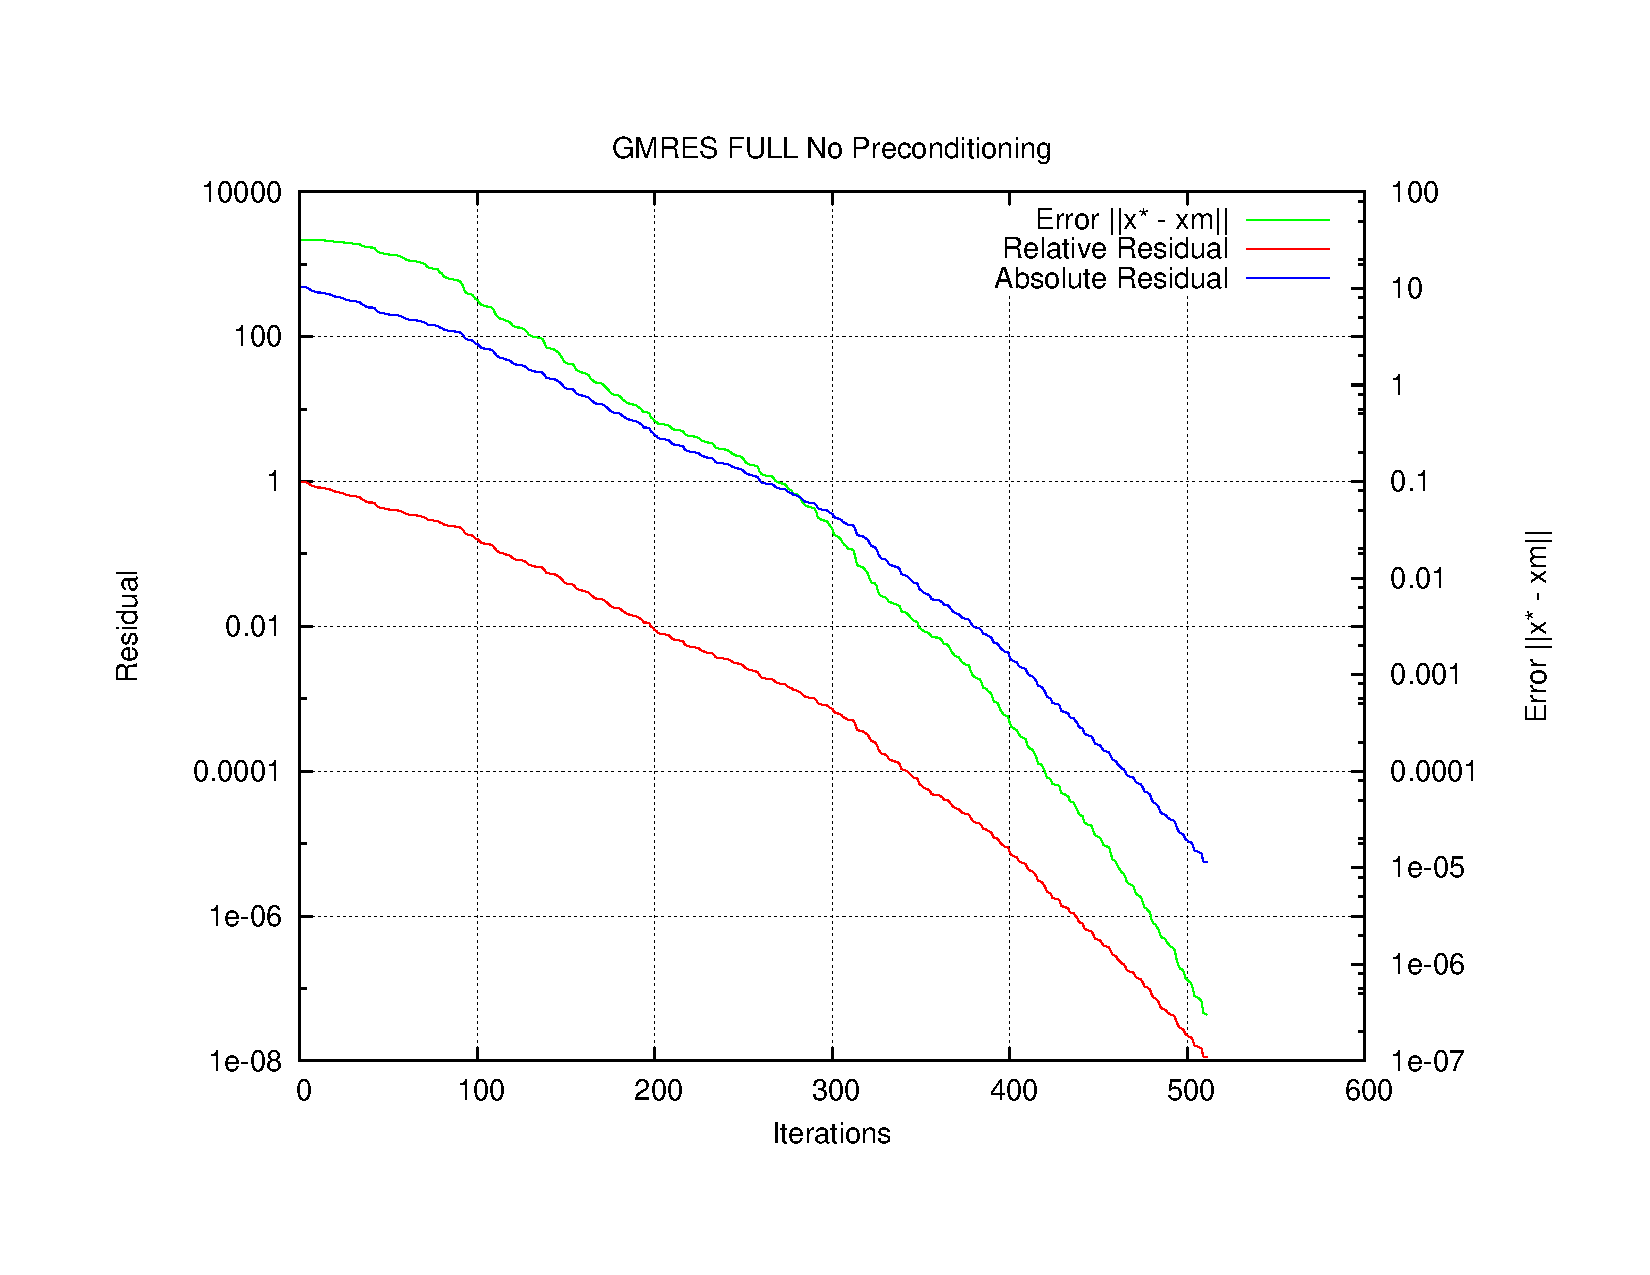
\includegraphics[scale=0.54]{./Output/GMRES_FULL_NO.pdf}\\
\caption{Plot 1: GMRES FULL No Preconditioning}}
\end{center}
\begin{center}
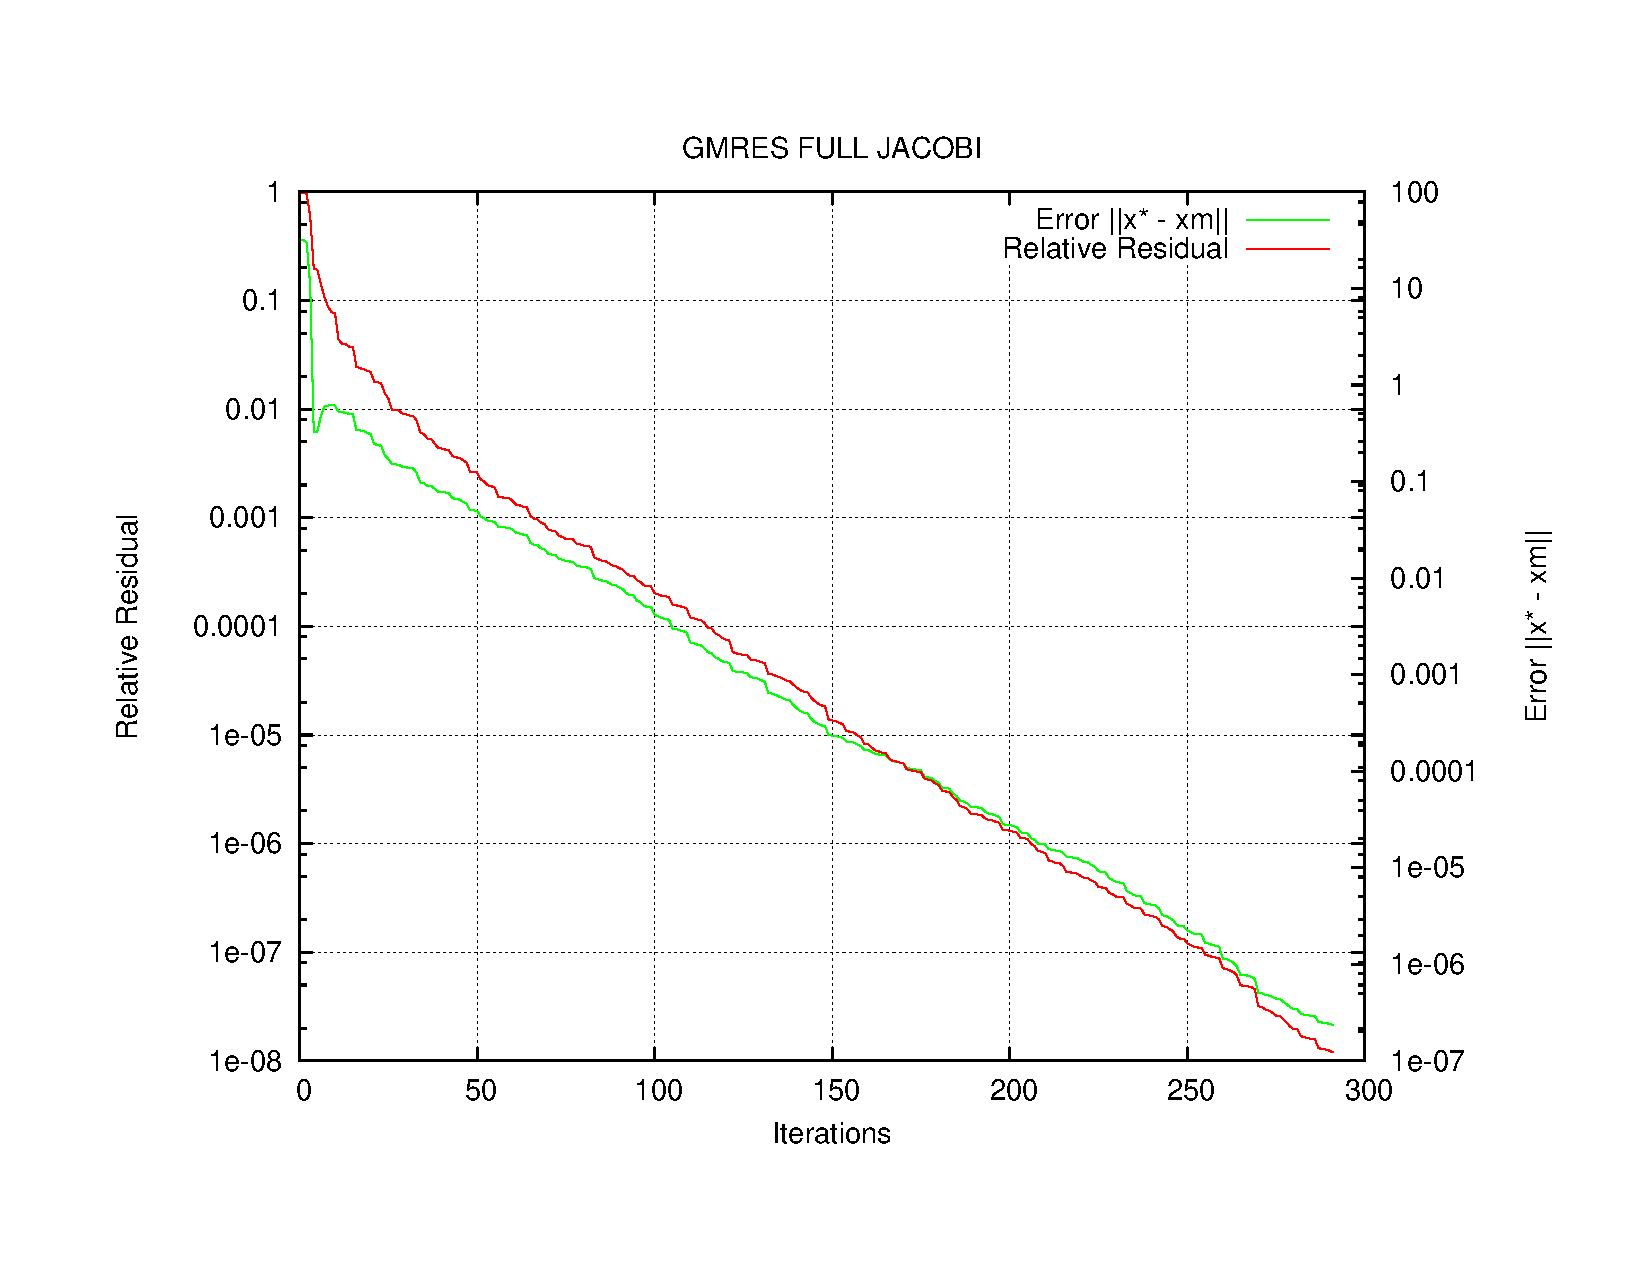
\includegraphics[scale=0.54]{./Output/GMRES_FULL_JACOBI.pdf}\\
\caption{Plot 2: GMRES FULL Jacobi Preconditioning}}
\end{center}
\begin{center}
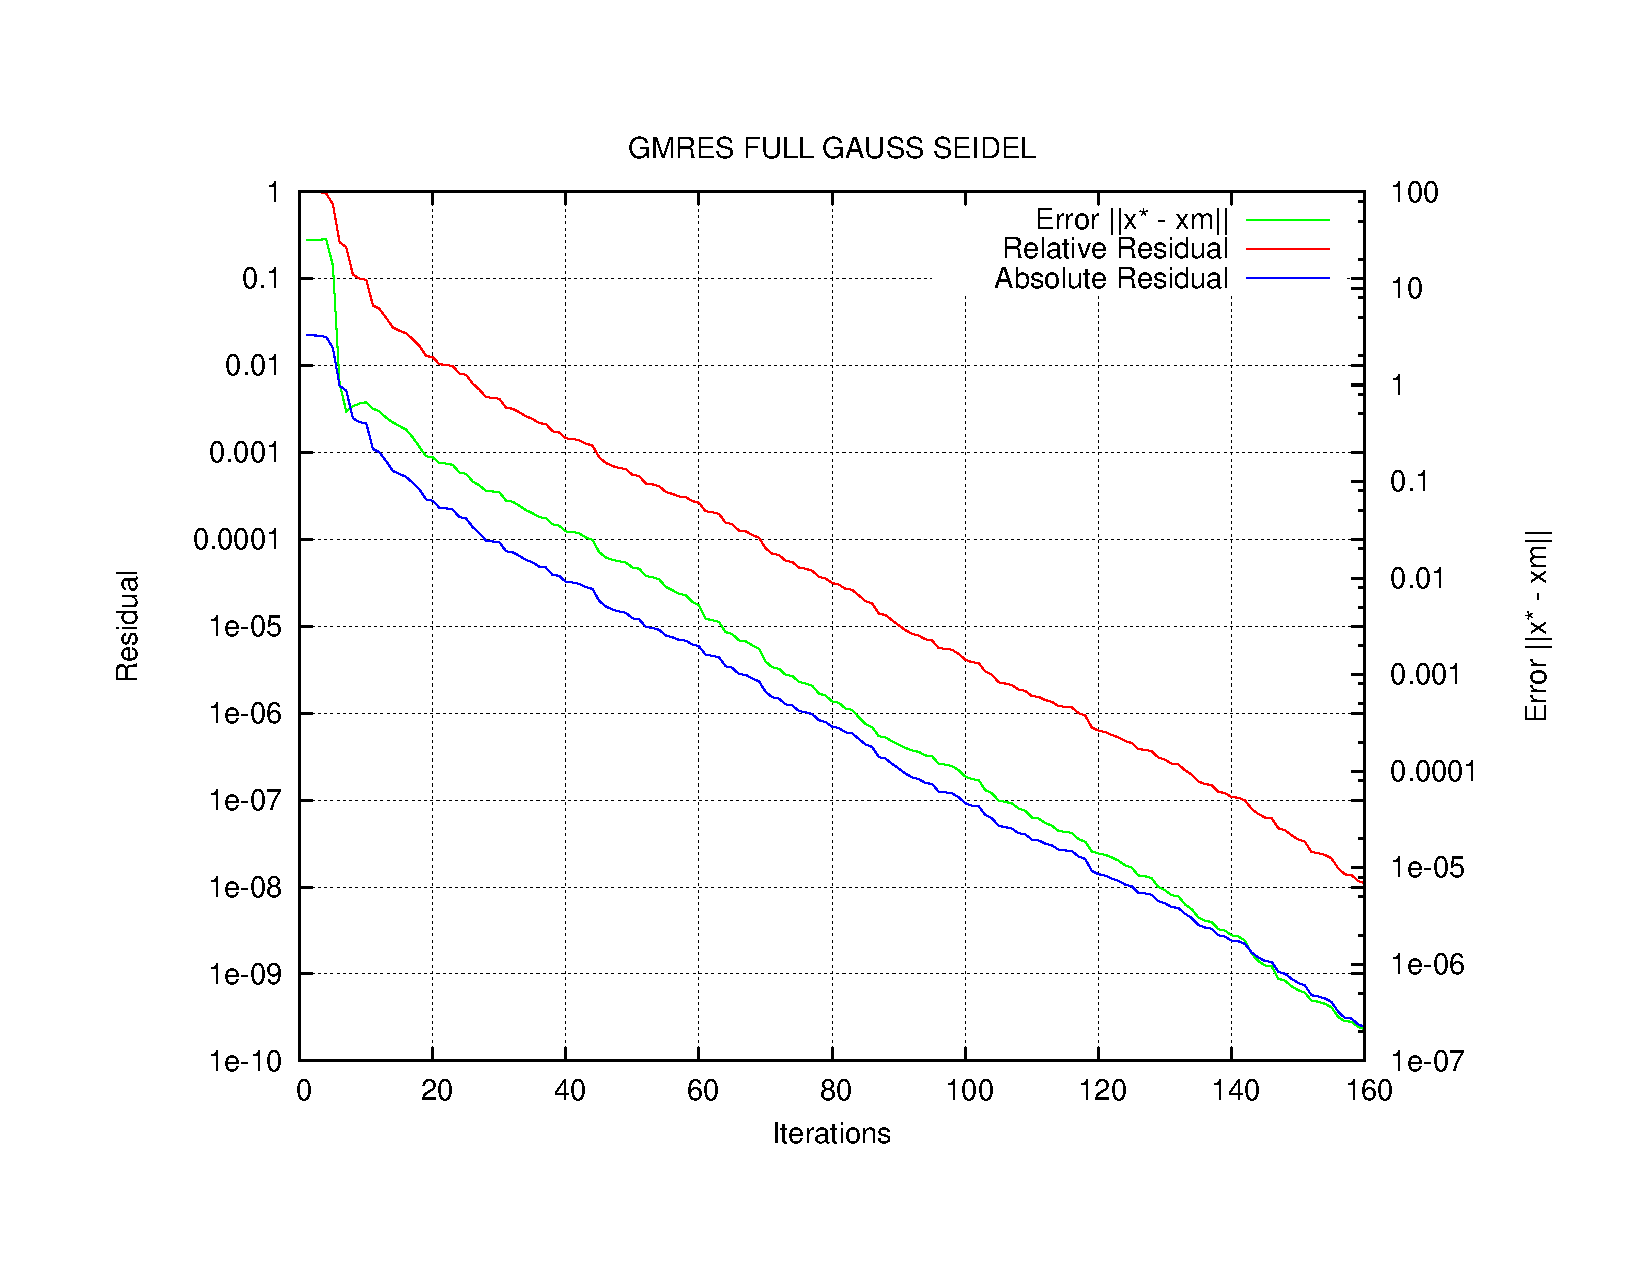
\includegraphics[scale=0.54]{./Output/GMRES_FULL_GAUSS_SEIDEL.pdf}\\
\caption{Plot 3: GMRES FULL Gauss Seidel Preconditioning}}
\end{center}
\begin{center}
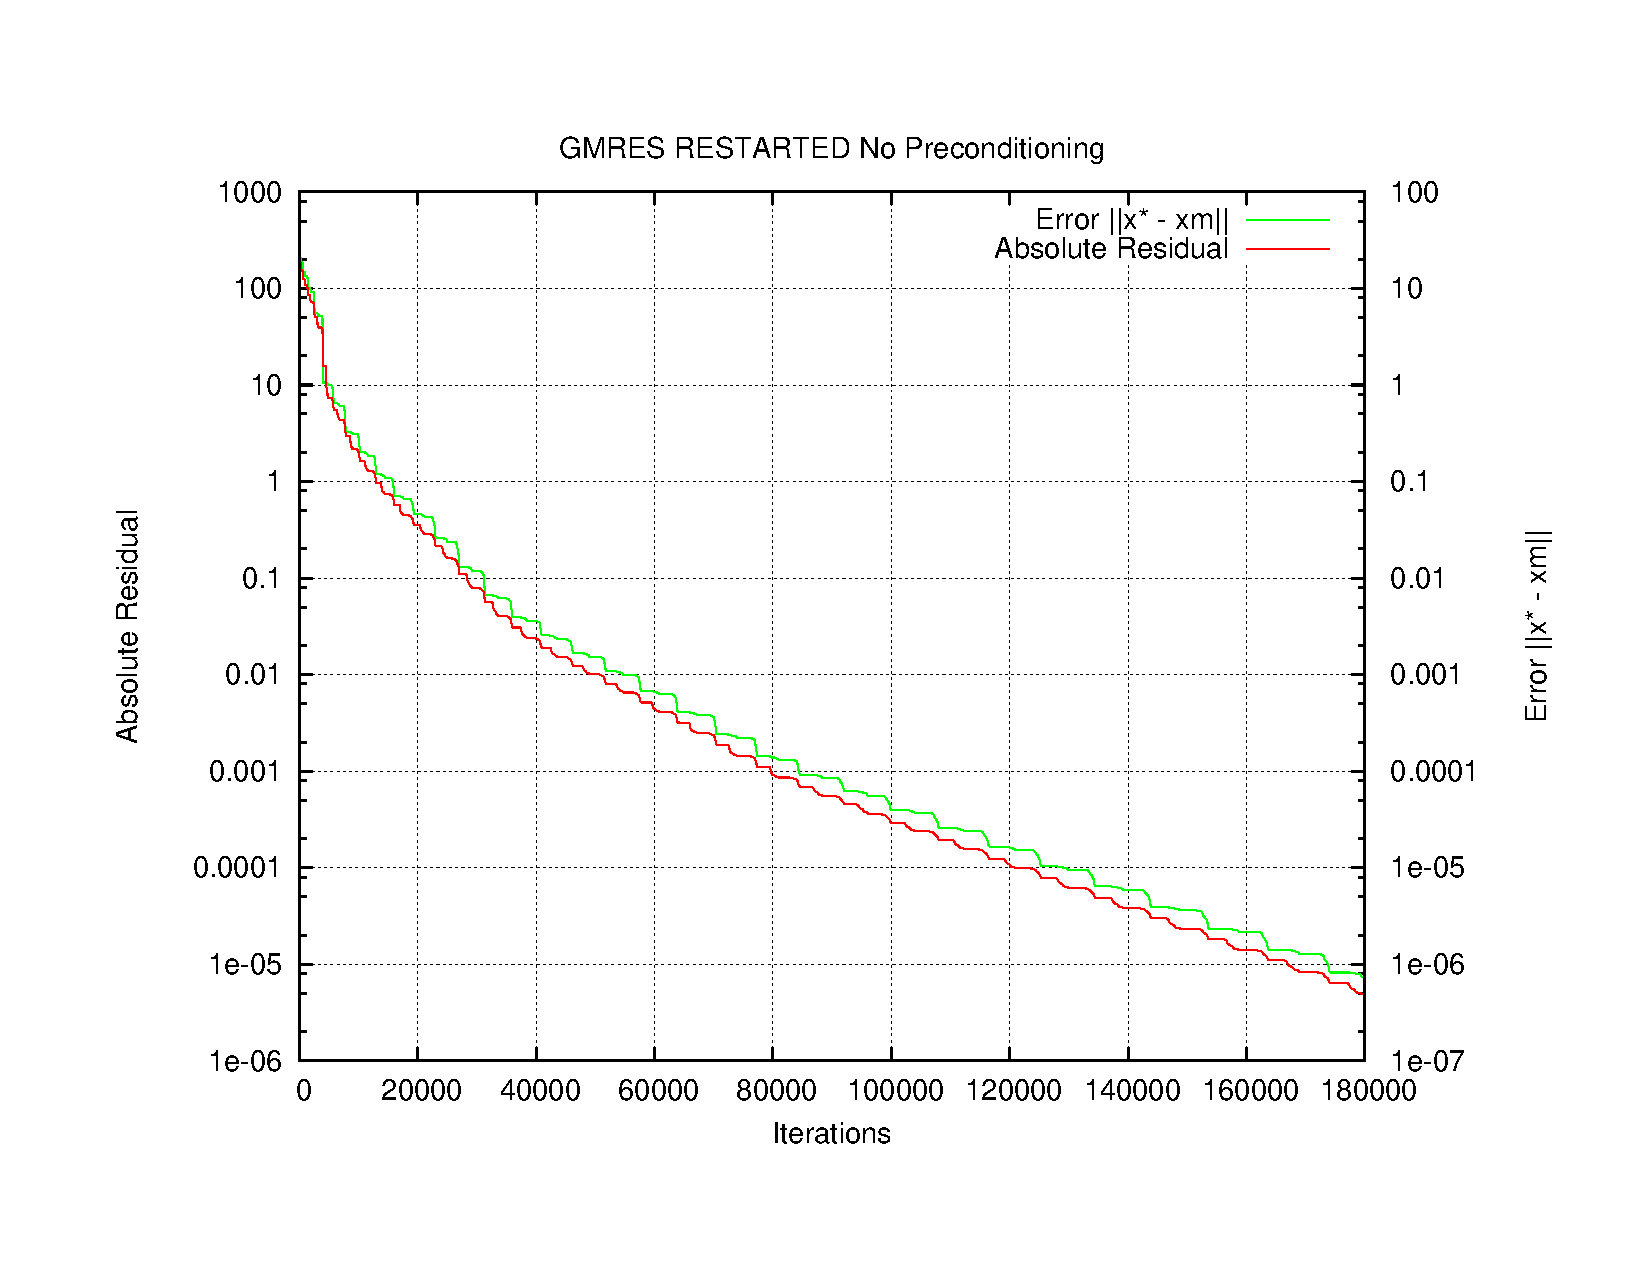
\includegraphics[scale=0.54]{./Output/GMRES_RESTARTED_NO.pdf}\\
\caption{Plot 4: GMRES RESTARTED No Preconditioning}}
\end{center}
\begin{center}
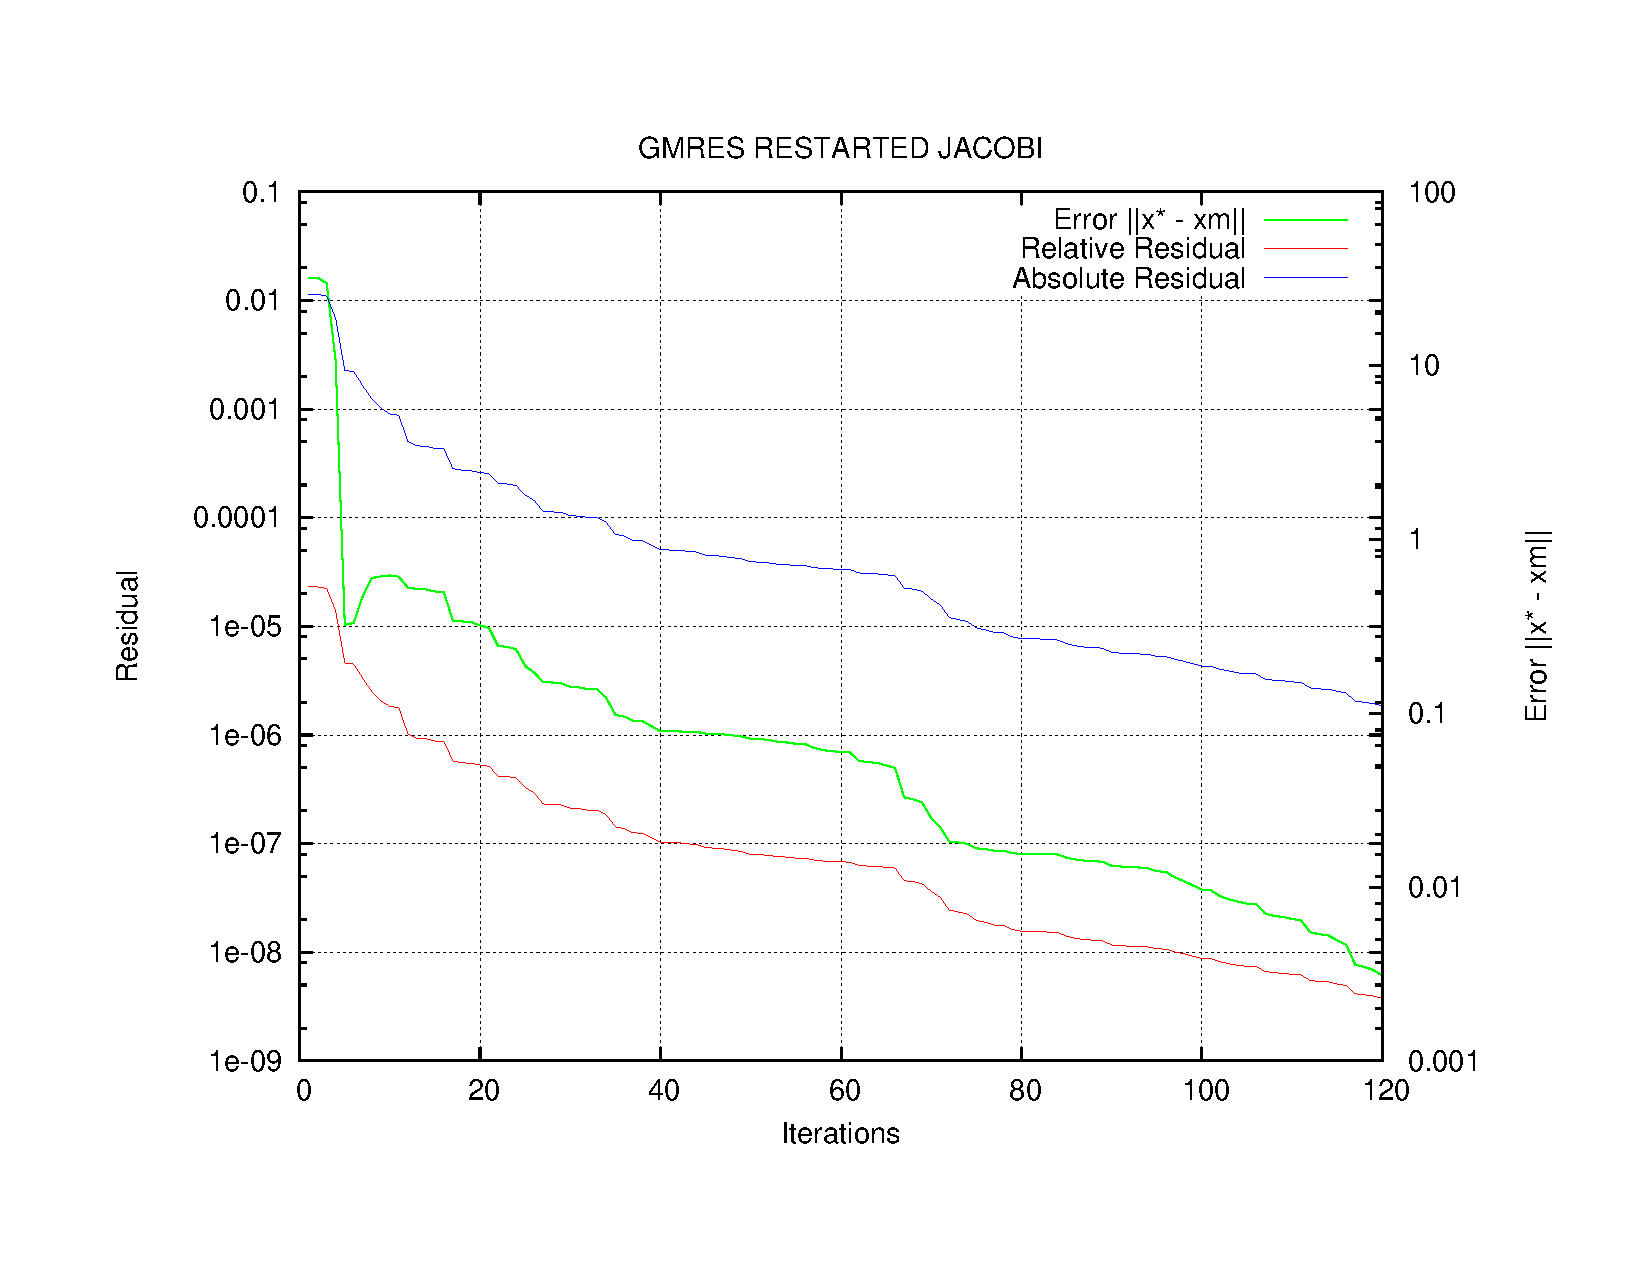
\includegraphics[scale=0.54]{./Output/GMRES_RESTARTED_JACOBI.pdf}\\
\caption{Plot 5: GMRES RESTARTED Jacobi Preconditioning}}
\end{center}
\begin{center}
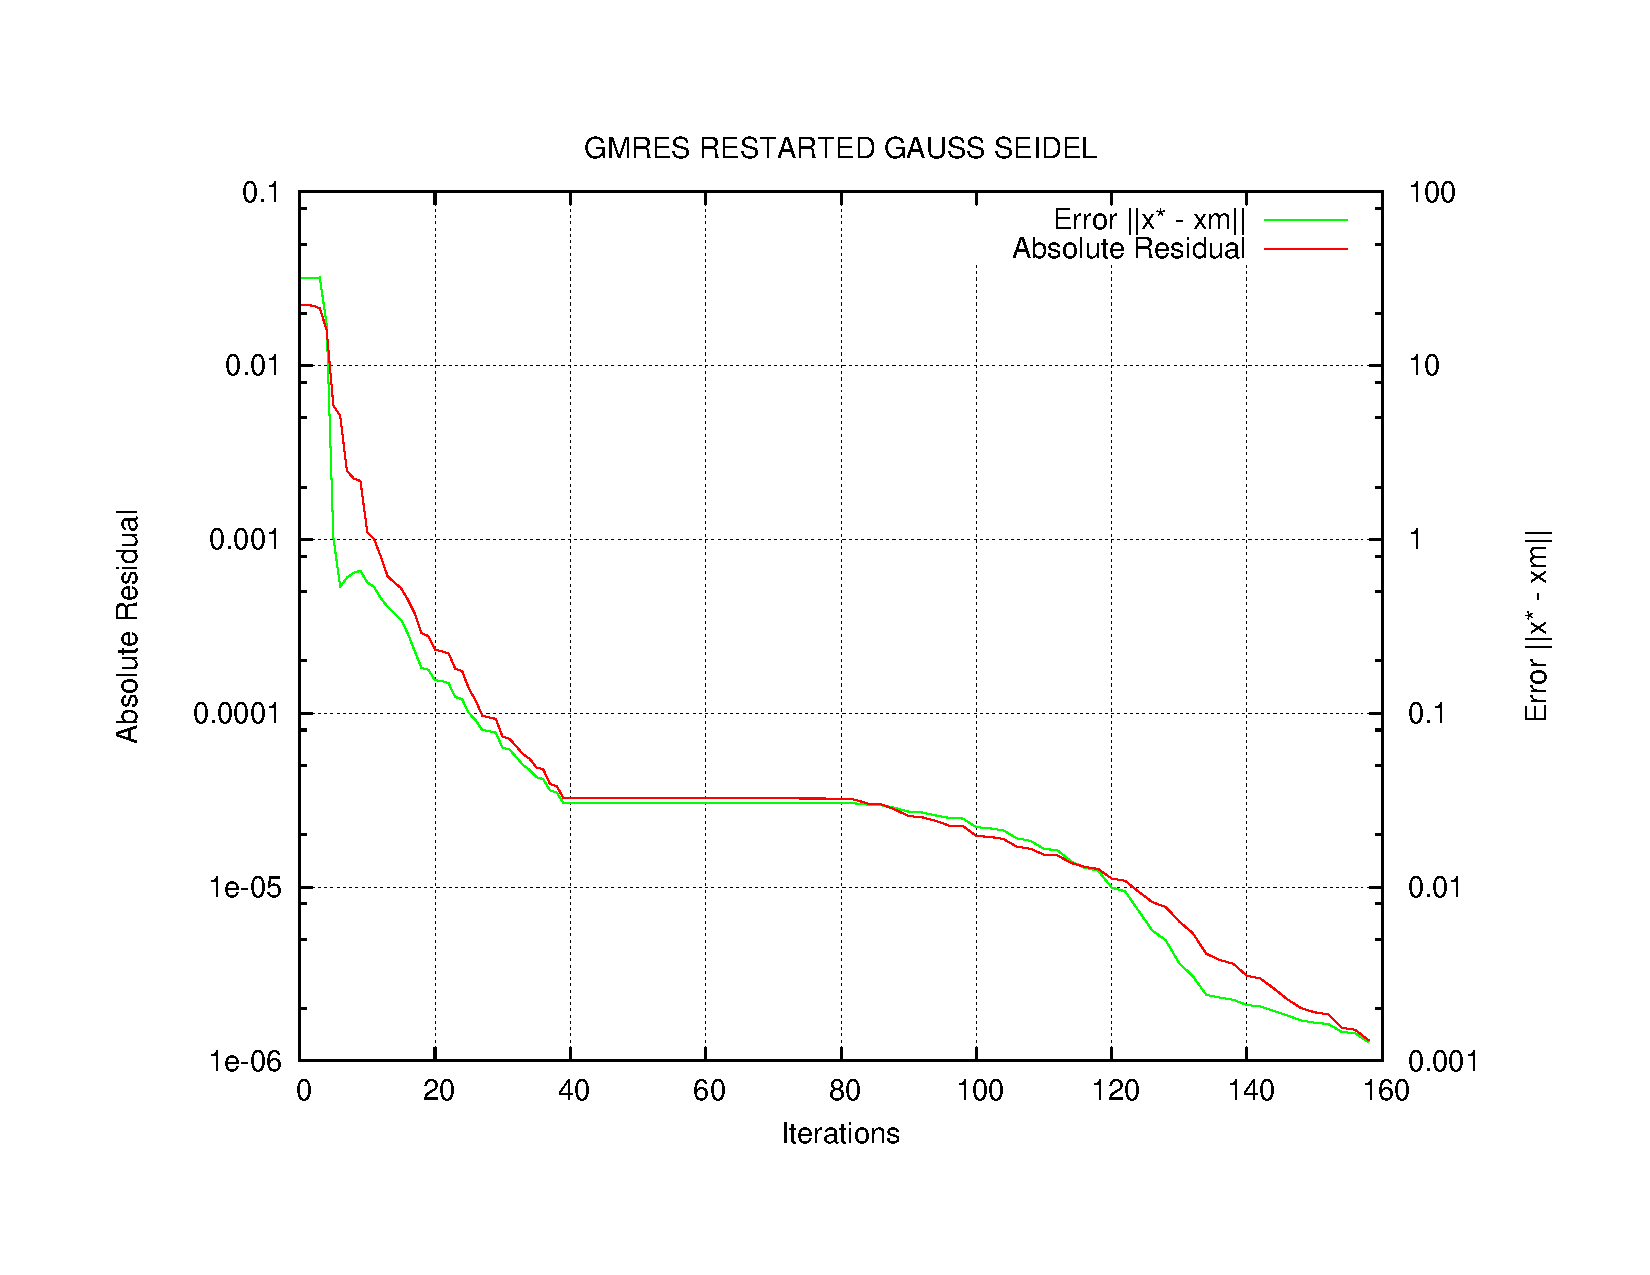
\includegraphics[scale=0.54]{./Output/GMRES_RESTARTED_GAUSS_SEIDEL.pdf}\\
\caption{Plot 6: GMRES RESTARTED Gauss Seidel Preconditioning}}
\end{center}
\begin{center}
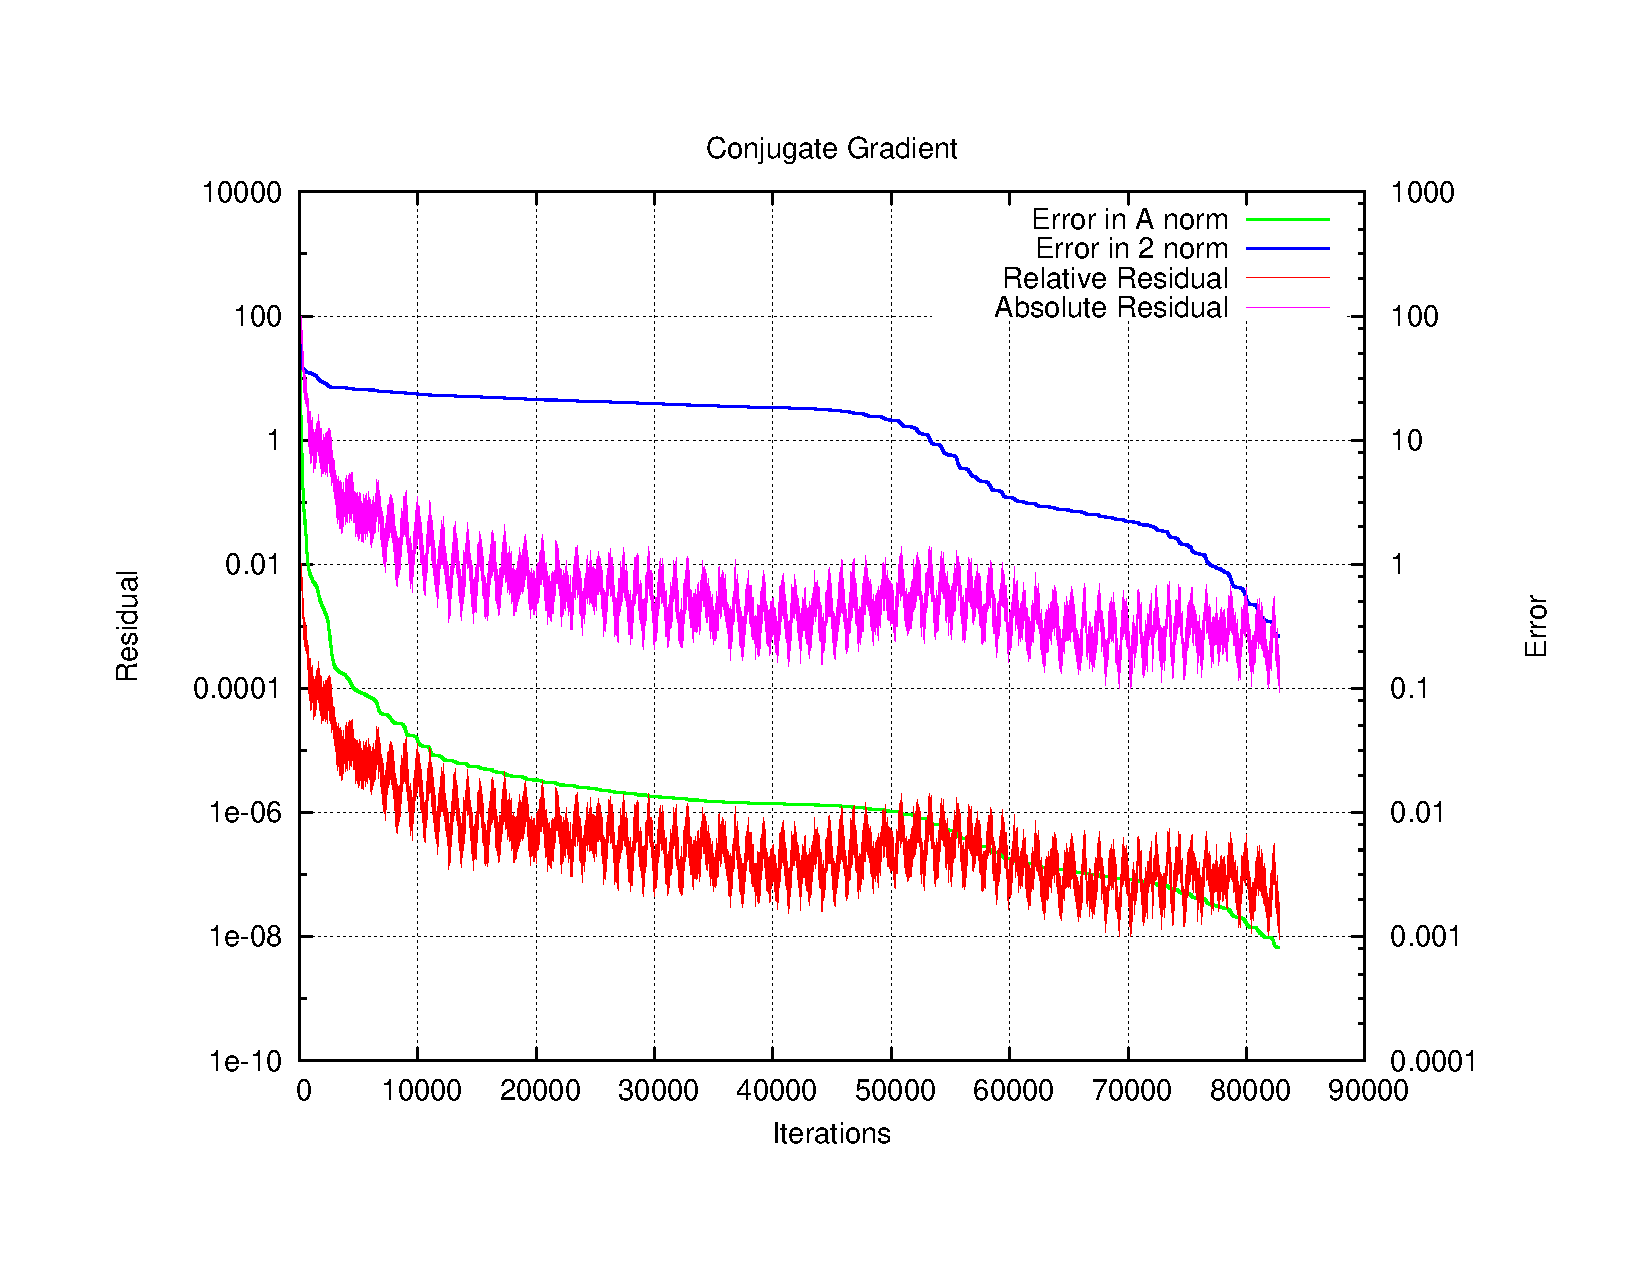
\includegraphics[scale=0.54]{./Output/CG.pdf}\\
\caption{Plot 7: Conjugate Gradient}}
\end{center}
\section{Full GMRES Method:}
Number of Krylov Vectors required: \textbf{512}
\section{Restarted GMRES Method:}
Best restart parameter (m) = 40 with time \sim 0.26-0.28 s
\\

This optimal method is faster than full GMRES method because the number of Krylov vectors is fixed to a lower number (40) than that required by full GMRES (512) which reduces the number of operations significantly[O(512^2)  to  O(40^2)].
\\

Additionally, the initial guess is improved at every execution of GMRES algorithm.
\section{Preconditioned GMRES Method:}
\begin{center}
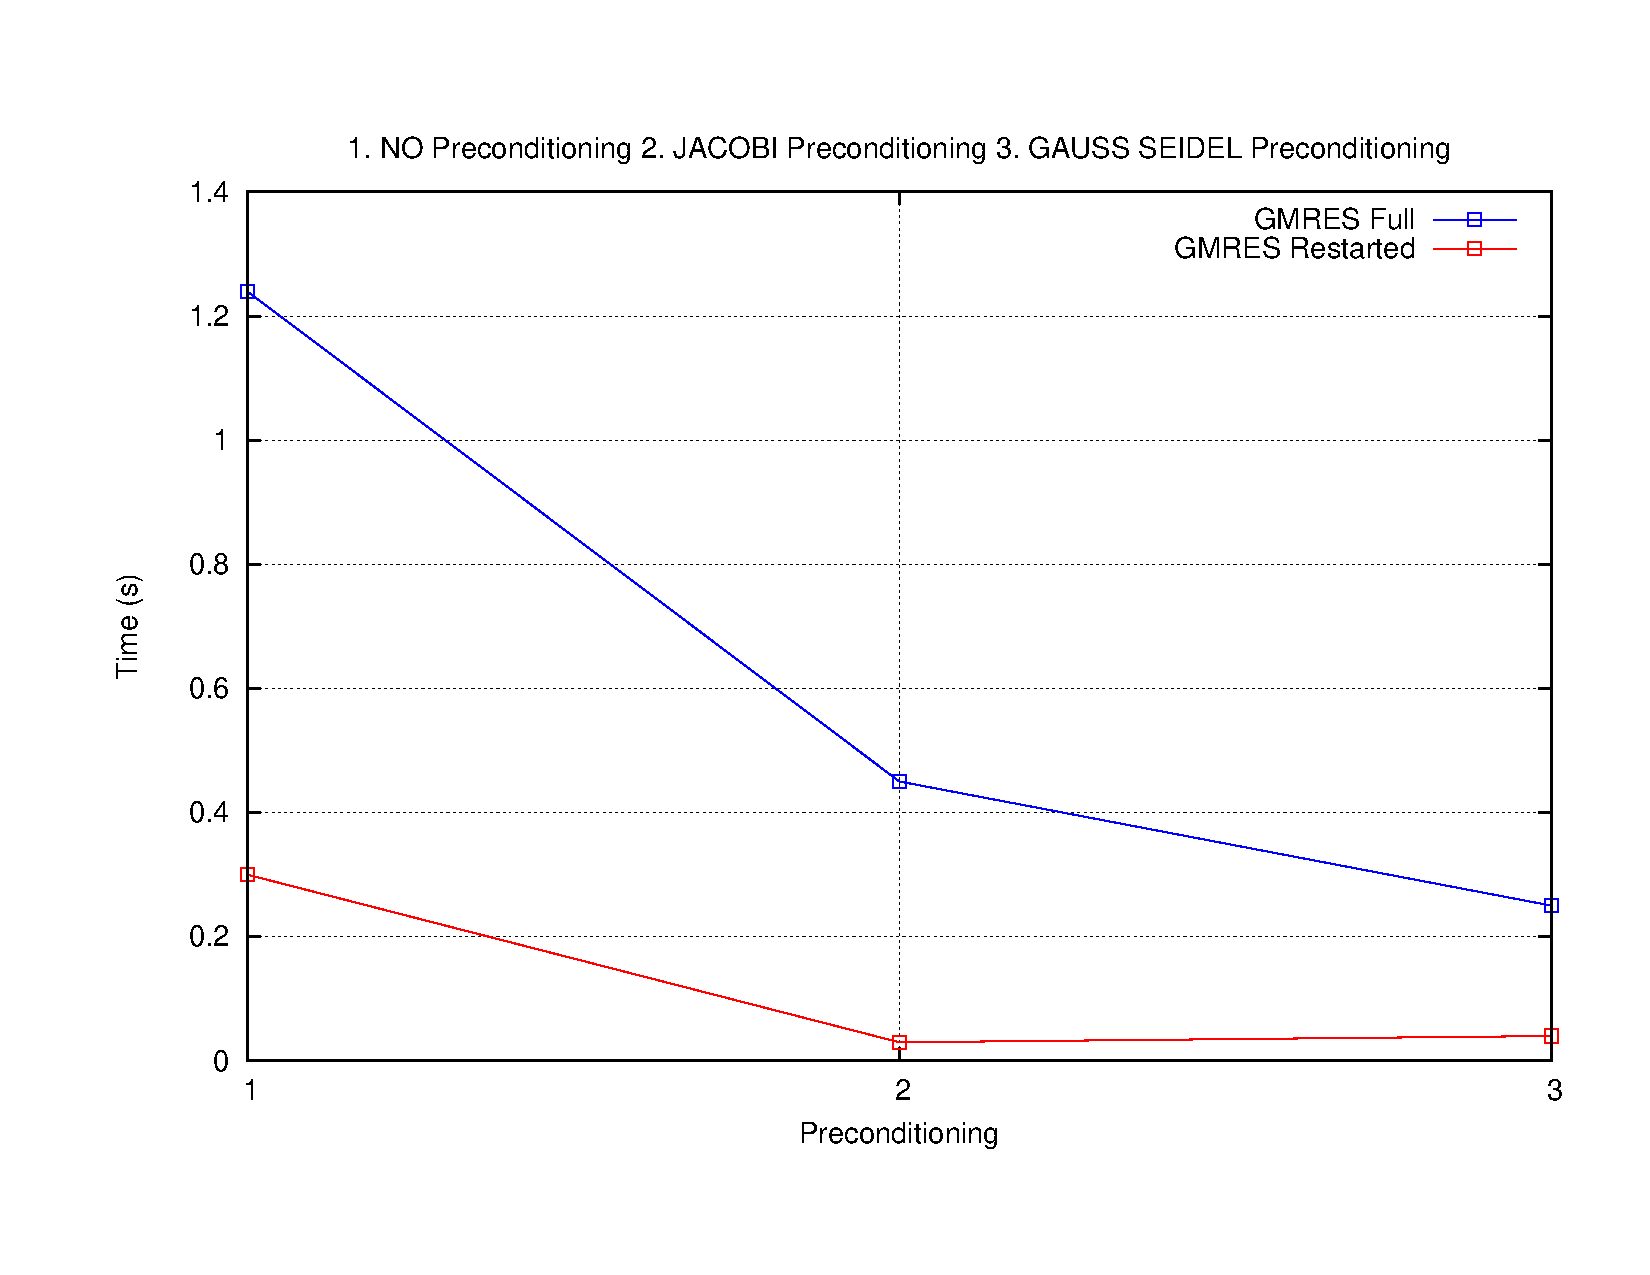
\includegraphics[scale=0.54]{./Output/Timings_GMRES.pdf}\\
\caption{Plot 8: Comparison of Timings with and without preconditioning}}
\end{center}
GMRES Method with Gauss Seidel preconditioning is the fastest one.
\\
Compare the true absolute residual r := b − Ax
with the residual of preconditioned system. Does the relative residual reduction depend on
which residual you monitor? (Why would one rather not monitor the true residual during
the computation of the solution?)

\section{Conjugate Gradient Method:}
Both the errors, i.e. error in A norm and error in 2 norm are plotted in Plot 7.
\\
Compare qualitatively the difference
in convergence behavior. (i.e. the difference between the two norms). Is there an explanation
for what you observe?
\end{document}